\subsection{Planos Tangentes e Aproximações Lineares e Diferenciais}

\subsubsection{Planos Tangentes}

Suponha que uma superfície $S$ tenha a equação $z = f(x, y)$, onde $f$ tenha derivadas parciais contínuas de primeira ordem e seja $P(x_0, y_0, z_0)$ um ponto na superfície S. pegue as curvas $C_1$ e $C_2$ que são respectivamente $f_x(x, y_0)$ e $f_y(x_0, y)$ seja $T_1, T_2$ retas tangentes as curvas $C_1, C_2$ obtemos um \textbf{Plano Tangente} a superfície $S$ no ponto $P$. 


\begin{figure}[H]
	\centering
	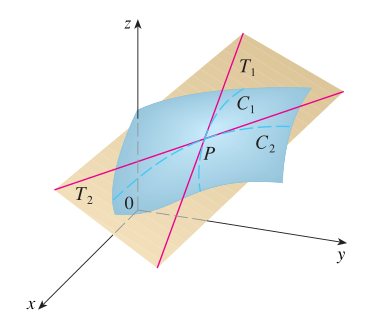
\includegraphics[width=0.4\linewidth]{pictures/plano.png}
	\label{fig:interpretacao}
	\caption{Plano Tangente Ao Ponto P}
\end{figure}

Temos que a equação do plano passando por $P(x_0, y_0, z_0)$ tem a forma: 

\begin{equation}
	A(x - x_0) + B(y - y_0) + C(z - z_0) = 0
	\label{equacao_plano_1}
\end{equation}

Dividindo em ambos os lados por -C temos 

\begin{equation}
	\dfrac{A}{-C}(x - x_0) + \dfrac{B}{-C}(y - y_0) + -z + z_0 = 0
	\label{equacao_plano_2}
\end{equation}

Escrevendo $a = -\dfrac{A}{C}$ e $b = -\dfrac{B}{C}$ temos 


\begin{equation}
	a(x - x_0) + b(y - y_0) = z - z_0 
	\label{equacao_plano_3}
\end{equation}

Repare que quando $y = y_0$ obtemos a seguinte equação 

\begin{equation}
	a(x - x_0) + b(y - y_0) = z - z_0 
	\label{equacao_plano_4}
\end{equation}

Se a equação \ref{equacao_plano_1} representa o plano temos que a equação \ref{equacao_plano_4} representa a reta $T_1$ logo sua inclinação é $a = f_x(x_0, y_0)$. 

De maneira análoga quando $x = x_0$ obtemos a seguinte equação:

\begin{equation}
	b(y - y_0) = z - z_0 
	\label{equacao_plano_5}
\end{equation}

Temos que a equação \ref{equacao_plano_5} representa a reta $T_2$ portanto sua inclinação é $b = f_y(x_0, y_0)$ o que motiva a seguinte definição 

\begin{definition} Sendo $f: \R^2 \rightarrow \R$ uma função onde suas derivadas parciais são contínuas uma equação do plano tangente a superfície $z = f(x, y)$ no ponto $P(x_0, y_0, z_0)$ é dada por 

\[
	z - z_0 = f_x(x_0, y_0)(x - x_0) + f_y(x_0, y_0)(y - y_0) 
\]
\end{definition}

\subsubsection{Aproximações Lineares}

Sabemos que a equação do plano do plano tangente ao gráfico de uma função $f$ cujas derivadas parciais são contínuas no ponto $(a, b, f(a, b))$ é 

\[
z = f(a, b) + f_x(a, b)(x - a) + f_y(a, b)(y - b) 
\]

Temos que a função linear cujo gráfico é esse plano tangente é 

\[
	L(x, y) = f(a, b) + f_x(a, b)(x - a) + f_y(a, b)(y - b) 
\]

Denominamos de \textbf{linearização} de $f$ em $(a, b)$ a aproximação: 

\[
	f(x, y) \approx f(a, b) + f_x(a, b)(x - a) + f_y(a, b)(y - b) 
\]

ou seja obtemos boas aproximações da função original através de $L(x,y)$ porém elas só ficam precisas em torno de $(a, b)$. o que motiva a seguinte definição 

\begin{definition} Sendo $f: \R^2 \rightarrow \R$ uma função onde suas derivadas parciais são contínuas temos que a aproximação em $(a, b)$ é dada da seguinte maneira 

\[
f(x, y) \approx f(a, b) + f_x(a, b)(x - a) + f_y(a, b)(y - b) 
\]

\end{definition}
%% adicionar dois exemplos com graficos no matplotlib 


\subsubsection{Diferenciais}

\paragraph{Uma variável.}
Seja $f:\mathbb{R}\to\mathbb{R}$ e fixe $x_0\in\mathbb{R}$. Dizemos que $f$ é derivável em $x_0$ se existe $f'(x_0)$ tal que, para $\Delta x\to 0$,
\[
\Delta y \;=\; f(x_0+\Delta x)-f(x_0) \;=\; f'(x_0)\,\Delta x \;+\; r(\Delta x),
\qquad \text{com } \frac{r(\Delta x)}{|\Delta x|}\longrightarrow 0.
\]
De forma equivalente (versão $\varepsilon$–$\delta$): 
\[
\forall\,\varepsilon>0\;\exists\,\delta>0\;\text{ tal que }\;|\Delta x|<\delta \;\Rightarrow\; 
\bigl|\Delta y - f'(x_0)\Delta x\bigr|\le \varepsilon\,|\Delta x|.
\]
O \emph{diferencial} de $f$ em $x_0$ é a aplicação linear dada por
\[
dy \;=\; f'(x_0)\,dx,
\]
onde $dx$ é um incremento independente. Assim, para $dx$ pequeno,
\[
f(x_0+dx) \;\approx\; f(x_0) + dy \;=\; f(x_0) + f'(x_0)\,dx.
\]

\paragraph{Duas variáveis.}
Seja $f:\mathbb{R}^2\to\mathbb{R}$ e fixe $(x_0,y_0)$. Dizemos que $f$ é \emph{diferenciável} em $(x_0,y_0)$ se existe uma aplicação linear 
\[
L(\Delta x,\Delta y)=a\,\Delta x + b\,\Delta y
\]
tal que, para $h=(\Delta x,\Delta y)\to(0,0)$,
\[
\Delta z \;=\; f(x_0+\Delta x,y_0+\Delta y) - f(x_0,y_0)
\;=\; L(\Delta x,\Delta y) \;+\; r(\Delta x,\Delta y),
\qquad \text{com } \frac{|r(\Delta x,\Delta y)|}{\sqrt{(\Delta x)^2+(\Delta y)^2}}\longrightarrow 0.
\]
Nessa situação, $a=f_x(x_0,y_0)$ e $b=f_y(x_0,y_0)$, de modo que o \emph{diferencial total} em $(x_0,y_0)$ é
\[
dz \;=\; f_x(x_0,y_0)\,dx \;+\; f_y(x_0,y_0)\,dy,
\]
e vale a aproximação de primeira ordem
\[
\Delta z \;=\; dz \;+\; o\!\left(\sqrt{(\Delta x)^2+(\Delta y)^2}\right).
\]
De forma equivalente (versão $\varepsilon$–$\delta$):
\[
\forall\,\varepsilon>0\;\exists\,\delta>0\;\text{ se }\sqrt{(\Delta x)^2+(\Delta y)^2}<\delta \;\Rightarrow\;
\left|\Delta z - \bigl(f_x(x_0,y_0)\Delta x + f_y(x_0,y_0)\Delta y\bigr)\right|
\le \varepsilon\,\sqrt{(\Delta x)^2+(\Delta y)^2}.
\]

\begin{definition}
	Seja $f:\mathbb{R}^2\to\mathbb{R}$. Diz-se que $f$ é \emph{diferenciável} em $(x_0,y_0)$ se existem números reais $a,b$ e uma função $r(\Delta x,\Delta y)$ tais que
	\[
	\Delta z \;=\; a\,\Delta x + b\,\Delta y \;+\; r(\Delta x,\Delta y),
	\qquad
	\frac{|r(\Delta x,\Delta y)|}{\sqrt{(\Delta x)^2+(\Delta y)^2}}\longrightarrow 0
	\quad\text{quando }(\Delta x,\Delta y)\to(0,0).
	\]
	Nesse caso, $a=f_x(x_0,y_0)$ e $b=f_y(x_0,y_0)$, e o diferencial total é $dz=f_x(x_0,y_0)\,dx+f_y(x_0,y_0)\,dy$.
\end{definition}

\begin{remark}
	(i) $dz$ é a parte \emph{linear} do incremento real $\Delta z$; por isso, em geral $\Delta z\neq dz$, mas $\Delta z - dz = o(\|( \Delta x,\Delta y)\|)$. 
	(ii) A mera existência das derivadas parciais não garante diferenciabilidade; um critério suficiente é a continuidade de $f_x$ e $f_y$ em uma vizinhança de $(x_0,y_0)$.
\end{remark}
